\section{Probabilistic programming with programmable inference in GenLite}

\begin{figure}[t]
\centering
    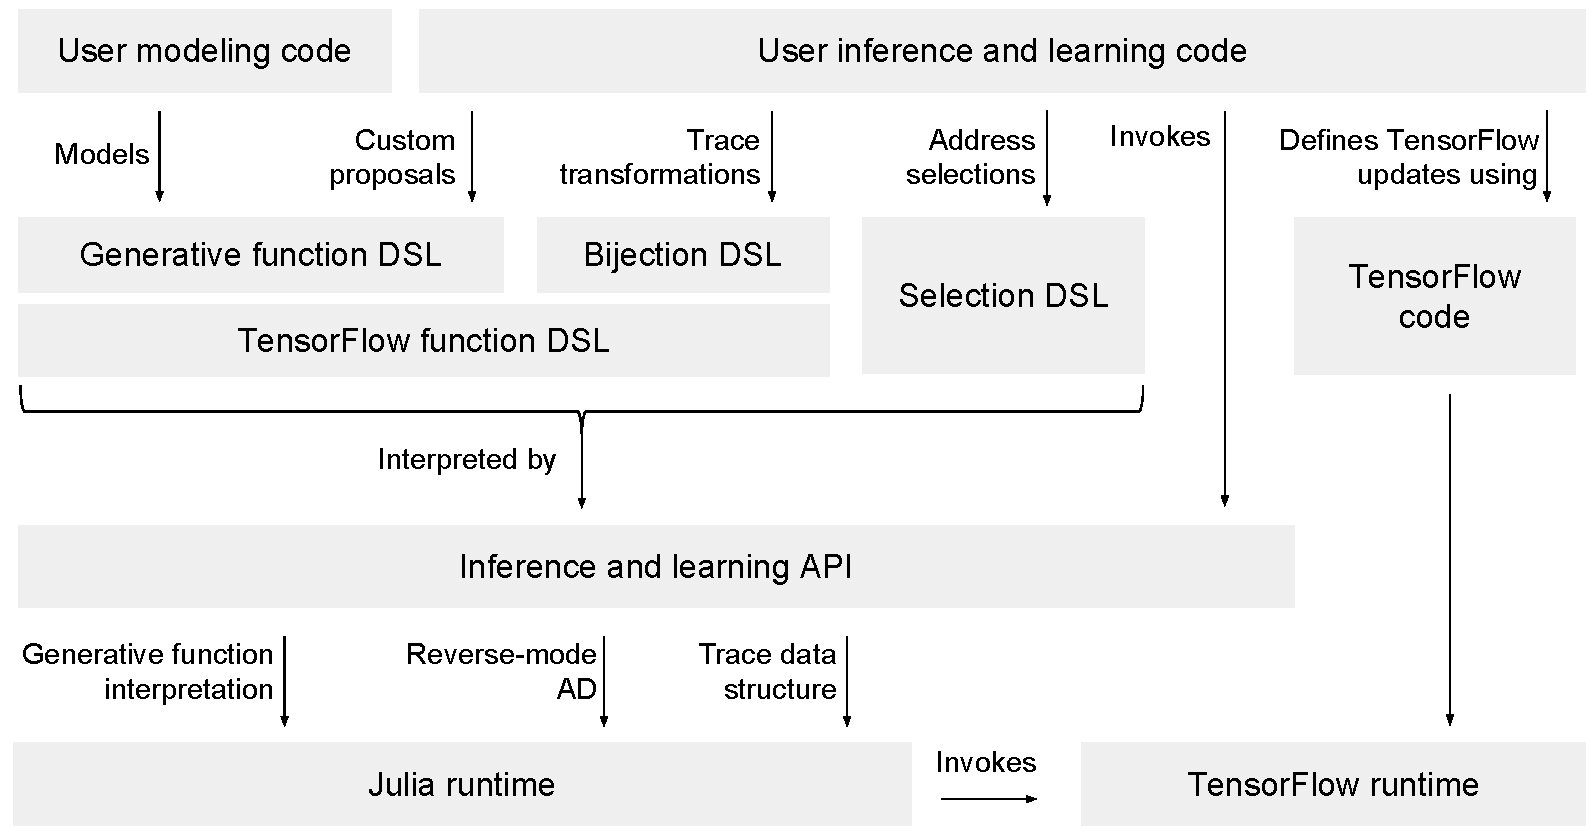
\includegraphics[width=\textwidth]{images/genlite-schematic.pdf}
    \caption{Architecture of GenLite including the TensorFlow extention}
    \label{fig:genlite-schematic}
\end{figure}

GenLite is a probabilistic modeling and inference platform implemented on top of Julia \cite{?}.
GenLite consists of a probabilistic programming language embedded in Julia, and an inference and learning API.
Users define generative models by writing \emph{generative functions}, which are Julia functions that are augmented with random choices that play the role of latent and observed random variables.
Unlike other probabilistic programming platforms, users implement inference algorithms in host language (Julia) code, building on high-level abstractions provided by the inference and learning API.
GenLite also contains auxiliary domain-specific languages for inference, which augment Julia functions with additional behavior and semantics:
First, \emph{selection functions} are used to identify subsets of random choices, and \emph{bijective functions} are used to define probability-preserving transformations between latent variable representations.
The remainder of this section provides additional details for those features of GenLite that are relevant to user-programmable inference based on deep learning.

\subsection{Generative functions}

A generative function is a Julia function annotated with $\gengen{}$.
A generative function behaves like a regular Julia function, except that it is functional with respect to its arguments (i.e. it should not mutate its arguments or any global state), and it has access to additional probabilistic language constructs.
Together these properties allow it to represent a probability distribution.
This section describes the additional language constructs.

\paragraph{Random choices and traces}
First, generative functions can make random choices (i.e. sample random values).
Random choices are typically drawn according to built-in or user-specified probability distributions.
For example the expression $\code{normal(mu, sig)}$ evaluates to a random draw from a normal distribution with mean $\code{mu}$ and standard-deviation $\code{std}$.
A random choice is typically assigned an \emph{address}, using the syntax $\code{@addr(normal(mu, std), addr)}$, where $\code{addr}$ is a dynamically computed string, or tuple of strings (which denote a hierarchical address).
Within every possible execution of the program, the random choices must have unique addresses.
Assuming that a generative function terminates (i.e. returns) with probability one\footnote{Verifying termination with probability one for arbitrary functions embeds the halting problem}, a generative function defines a probability distribution on \emph{traces}, which are associative collections that map the address of a random choice to its value.
In the simple setting where the set of addresses that are sampled is constant across all executions, the GenLite function denotes a joint distribution on a collection of random variables identified with addresses.
A formal semantics for GenLite generative functions is outside the scope of this paper.
Informally, the probability of a certain trace is the product of the probability that each address was assigned its given value in the trace, if the trace is the result of some possible execution of the program, and zero otherwise.
We denote the probability of a trace $t$ for generative function $p$ by $p(t)$.
When continuous random choices are included, a generative function that terminates with probability one denotes a probability measure on traces.
See \cite{CusumanoPLDI2018} and \cite{Borgstrom} for examples of trace-based semantics for probabilistic programming languages.
Finally, note that not all random choices made by a generative function need to be assigned addresses---random choices without addresses are called \emph{untraced}.
The ability to make untraced random choices means that GenLite functions can invoke arbitrary black box code.

\paragraph{Reading from an input trace}
Each generative function defines a distribution on its own trace.
In addition, a generative function may optionally read from an \emph{input trace}, using the syntax $\code{@read(addr)}$, where $\code{addr}$ is a dynamically computed string or tuple of strings.
As will be discussed in more detail below, input traces enable generative functions to be used to define proposal distribution in Markov chain Monte Carlo (MCMC) and importance sampling and sequential Monte Carlo inference algorithms.

\paragraph{Trainable static parameters}
Generative functions can also contain \emph{trainable static parameters}.
These parameters are declared at the beginning of the generative function definition using the syntax $\code{@param name}$ or, with an optional type declaration: $\code{@param name::type}$.
These parameters are static in the sense that all invocation of the generative function make use of the same values for these parameters.
The values of static parameters are set by the user in Julia code, using the API method $\code{set\_param!(gf, name, value)}$, where $\code{gf}$ is a reference to the generative function.
Gradients with respect to static parameters are obtained by the user with $\code{get\_param\_grad(gf, name)}$.
Gradients are discussed in more detail below in the section on training generative functions (Section~\ref{sec:training}).

\paragraph{Calling other generative functions}
Finally, generative functions can invoke other generative functions, in three ways:
First, a generative function may make an \emph{untraced invocation}, using regular function invocation syntax (e.g. $\code{fn(args..)}$).
Second, a generative function may invoke a generative function using the syntax $\code{@addr(fn(args...), addr)}$, which indicates that the entire trace of the function $\code{fn}$ should be placed in a sub-trace of the current function's trace, under namespace $\code{addr}$.
Third, a generative function may use $\code{@splice(fn(args...), addr)}$, which indicates that the trace of $\code{fn}$ should be spliced into the current trace, without introducing a separate namespace.
It is an error if any addresses in the trace of $\code{fn}$ collide with any address assigned by the caller.
The use of $\code{@addr}$ to make random choices, combined with its use to invoke other generative functions, means that the trace of a generative function is in general a hierarchical data structure.

\subsection{Selection functions}

\subsection{High-level embedded inference programming}

\subsubsection{Traces are user-space Julia values}

\subsubsection{Observation traces}

\subsubsection{Monte Carlo inference operators}

% imp, imp2, mh, mh2

% the full set of inference operators, and the semantics of these operators, are outside the scope of this paper

\subsubsection{Training generative functions using $\genbackprop{}$} \label{sec:training}

\subsubsection{Gradient-based MAP using $\gentracegrad{}$}

GenLite \cite{TODO} is a flexible probabilistic programming language designed to support user-programmable inference.
This section provides a very brief introduction to GenLite.
GenLite is embedded in Julia \cite{TODO}.
In GenLite, users first express a probabilistic generative model as a \emph{generative function}, which is written in an embedded DSL that extends Julia functions with the ability to make traced random choies.
Then, users implement Monte Carlo inference algorithms for the model in Julia code, drawing heavily on GenLite's inference programming API, which provides core data structures and inference primitives that utilize the programmatic representation of the generative model.
User inference code is written at a higher level of abstraction than typical custom sampler implementations, which makes it more efficient to develop, maintain, and reason about.

In GenLite, a \emph{trace} is a Julia value (of type \texttt{Trace}) that contains a record of random choices made by some generative function.
Generative functions, which are declared with keyword \texttt{@gen function}, extend Julia with four language constructs:
\begin{enumerate}
\item \texttt{@rand(<expr>, <address>)}: Sample a random value (i.e. a `random choice') from probability distribution \expr{}, where \address{} is a string or tuple of strings that specify a hierarchical name, or `address' for the random choice.
Record the random choice in the trace at the given address.
\item \texttt{@call(<expr>, <address>)}: Invoke a generative function given by \expr{}, and record the resulting trace for the invoked function under address \address{} in the current trace.
\item \texttt{@read(<address>)}: If an input trace is provided, read the value in the input trace at the given \address{}.
This feature is used by generative functions that represent proposal distributions (see below).
\item \texttt{@param <name>::<type>}: Declare a trainable parameter of a generative function, which is static (i.e. the same value is shared by all invocations of the generative function).
Static parameters are initialized by the user outside of the generative function body.
\end{enumerate}

Note that generative functions can contain arbitrary Julia code.
Figure~\ref{fig:model-code-figure} shows a generative function that only exercises the \texttt{@rand} keyword.
In addition to generative models, proposal distributions for MCMC and importance sampling can also be expressed as generative functions \cite{cusumano2018using}.

The GenLite inference programming API contains a number of methods that implement building blocks for inference and learning algorithms.
A building block that is used for training the static parameters of generative functions is \texttt{backprop}, which has the following type signature:
\begin{center}
    \texttt{backprop(fn::GenerativeFunction, args::Tuple, trace::Trace, [input\_trace::Trace])}
\end{center}
The trace must be a complete trace of the given generative function for the given arguments to the function.
This method computes the gradient of the log probability of the trace with respect to all static parameters, using reverse-mode automatic differentiation (AD).
Each static parameter has a \emph{gradient accumulator}, which is a value that is incremented by the gradient during each call to \texttt{backprop}.
User Julia code reads and write to the gradient accumulator values and the values of static parameters to perform parameter updates, using GenLite methods:\\
\texttt{set\_param!(fn::GenerativeFunction, name::Symbol, value)}\\
\texttt{get\_param(fn::GenerativeFunction, name::Symbol)}\\
\texttt{get\_param\_grad(fn::GenerativeFunction, name::Symbol)}\\
\texttt{zero\_param\_grad!(fn::GenerativeFunction, name::Symbol)}

